% !TEX encoding = UTF-8 Unicode

\documentclass[11pt]{beamer}

\usepackage{color}
\usepackage{url}
\usepackage{amsthm}
\usepackage[T2A]{fontenc} % enable Cyrillic fonts
\usepackage[utf8]{inputenc} % make weird characters work
\usepackage{graphicx}
\usepackage{subcaption}
\usepackage{amsmath}
\usepackage{comment}
% \graphicspath{ {.} }

\usepackage[english,serbian]{babel}
%\usepackage[english,serbianc]{babel} %ukljuciti babel sa ovim opcijama, umesto gornjim, ukoliko se koristi cirilica

%\usepackage[unicode]{hyperref}
%\hypersetup{colorlinks,citecolor=green,filecolor=green,linkcolor=blue,urlcolor=blue}

\newtheorem*{tvrdjenje}{Tvrđenje}
\newtheorem*{hipoteza}{Hipoteza}
\theoremstyle{definition}
%\newtheorem{primer}{Пример}[section] %ćirilični primer
\newtheorem{primer}{Primer}[section]

\mode<presentation>{\usetheme{Warsaw}}
%\usecolortheme{lily}
\usefonttheme{serif}

%\AtBeginSection[]{
%\begin{frame}
%\frametitle{Sadržaj}
%\tableofcontents[currentsection]
%\end{frame}
%}

\title{Primena mašinskog učenja u verifikaciji softvera}

\author[\hspace{-0.8em}N. Dimitrijević, R. Đorđević, L. Živanović, D. Špadijer]
		{Nikola Dimitrijević\\ % \footnote{nikoladim95@gmail.com}\\
        Rastko Đorđević\\ % \footnote{mi14078@alas.matf.bg.ac.rs}\\
        Luka Živanović\\ % \footnote{mi14164@alas.matf.bg.ac.rs}\\
        Dimitrije Špadijer} % \footnote{mm11021@alas.matf.bg.ac.rs}\\}
\date{14. maj 2018.}

\begin{document}
\begin{frame}
\titlepage
\end{frame}

\section[]{Uvod}
\label{sec:uvod}
\begin{frame}
\frametitle{Uvod}
\begin{itemize}
\item Softverska rešenja su prisutna svuda
\item Avioni, samovozeći automobili, medicinski uređaji
\item Veoma je važno da taj softver bude ispravan
\item Verifikacija softvera se bavi proverom ispravnosti softvera
\item Mašinsko učenje je popularno i s puno uspeha
\item Primene mašinskog učenja u verifikaciji
\end{itemize}
\end{frame}

\section{Mašinsko učenje}

\begin{frame}
\frametitle{Mašinsko učenje}

\begin{block}{Definicija}
\textcolor{red}{Mašinsko učenje} bavi se proučavanjem indukcije, odnosno generalizacije, čime formalizuje uopštavanje od uzorka određene veličine ka univerzalnim zaključcima.
\end{block}

\begin{itemize}
\item Mašinsko učenje postiže rezultate superiorne u odnosu na rezultate ljudskih eksperata
\item Pogodno za probleme koji se teško definišu, a izuzetno lako rešavaju, i u kojima je prihvatljiva poneka greška
\item Kako se primenjuje na verifikaciju, ako se dopuštaju greške?
\end{itemize}
\end{frame}

%ml slika
{
\begin{frame}{}
 	\begin{center}
         	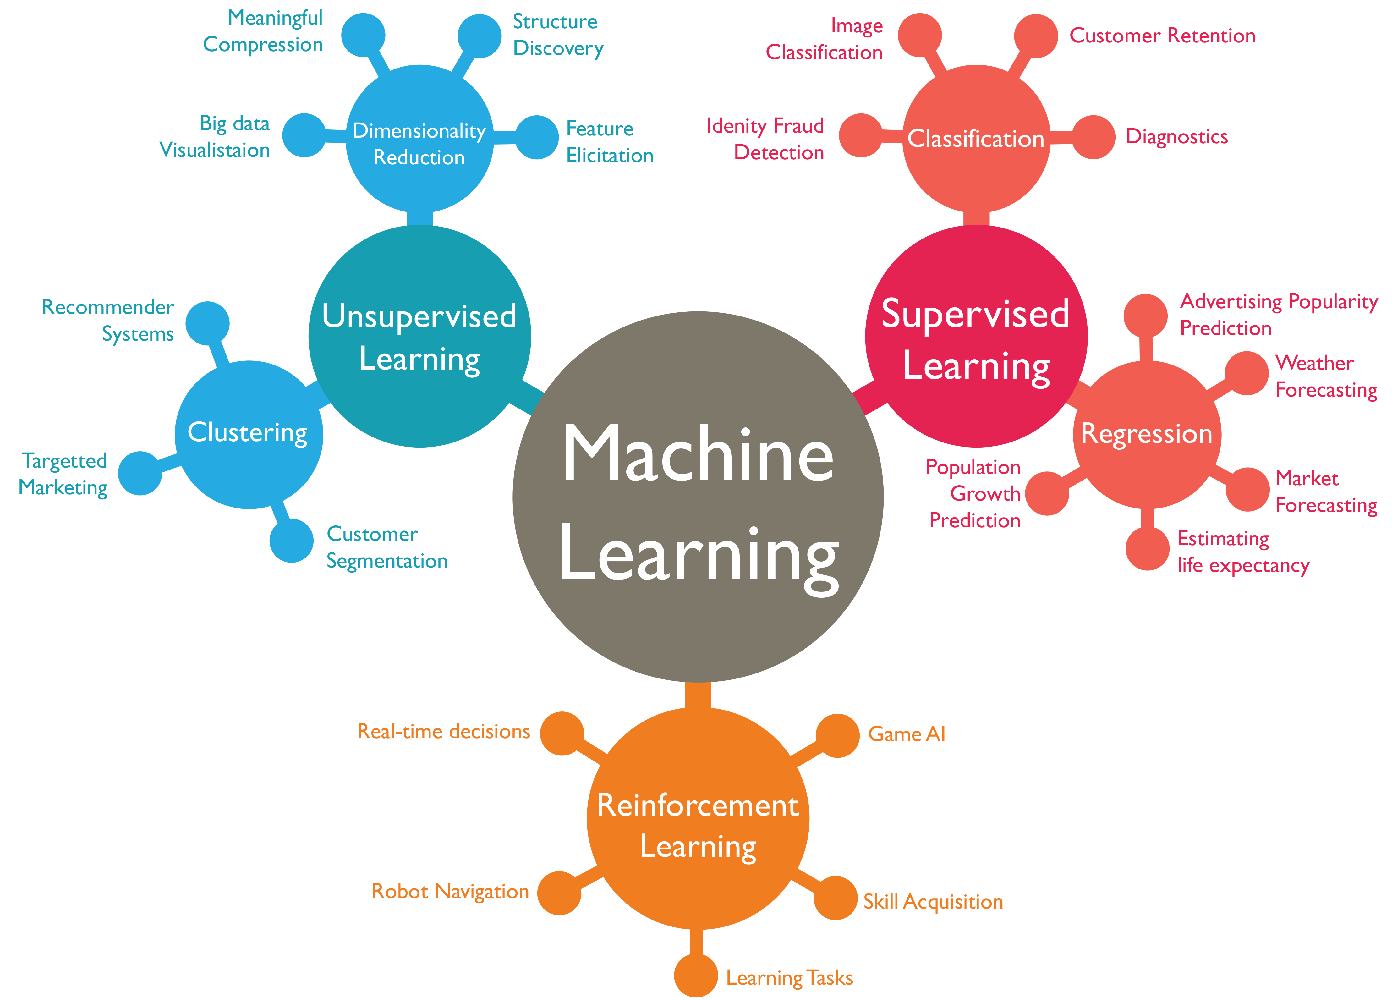
\includegraphics[width=\textwidth,height=0.9\textheight,keepaspectratio]{machine-learning.png}
        \end{center}
\end{frame}


\section{Verifikacija softvera}
\label{sec:verifikacija}
\begin{frame}
\frametitle{Verifikacija softvera}
\begin{itemize}
\item Oblast razvoja softvera koja se bavi proverom ispravnosti softvera
\item Potpuno ispravan i delimično ispravan softver
\item Razlika je u tome da li se zaustavlja za svaki ulaz
\item Zbog neodlučivosti halting problema, uglavnom se proverava delimična ispravnost
\item Dinamička i statička verifikacija
\end{itemize}
\end{frame}

\begin{frame}
\frametitle{Verifikacija softvera}
\begin{itemize}
\item Dinamička verifikacija:
	\begin{itemize}
		\item Provera ispravnosti softvera tokom njegovog izvršavanja
		\item Testiranje $\subset$ dinamička verifikacija
		\item Testiranjem se dokazuje prisustvo, ali ne i odsustvo grešaka
		\item Dobar skup testova obezbeđuje sigurnost i poverenje u softver
		\item Debagovanje --- drugi najčešći vid dinamičke verifikacije
	\end{itemize}
\item Statička verifikacija:
	\begin{itemize}
		\item Provera ispravnosti softvera bez njegovog pokretanja
		\item Pregled koda i automatska verifikacija
		\item Uvid u kvalitet koda i u propuste
	\end{itemize}
\end{itemize}
\end{frame}

\section{Odabrani problemi verifikacije}
\label{sec:naslovN}

\subsection{Formalna verifikacija softvera}
\label{subsec:formalna-verifikacija}
\begin{frame}
\frametitle{Formalna verifikacija}
\begin{itemize}
\item Formalni, matematički pristup verifikaciji
\item $P$ program, $T$ skup testova, $S$ specifikacija
$$(\forall t\in T)\ [prolazi(P,t)\wedge S\models t]\Rightarrow P\equiv S$$
\item Dva česta problema:
	\begin{itemize}
	\item Pronaći \textcolor{red}{adekvatan} skup testova $T$
	\item Proveriti tačnost konjunkcije $prolazi(P,t)\wedge S\models t$ (\textcolor{red}{problem proročišta})
	\end{itemize}
\item Prevazilaze se primenom mašinskog učenja i indukovanjem teorije koja odgovara datim podacima
\item Matematički pojmovi iz teorije jednačina (eng. \textcolor{red}{equational theory})
\end{itemize}
\end{frame}

\begin{frame}
\frametitle{Formalna verifikacija}
\begin{itemize}
\item Centralni pojam je $\Sigma$-teorija; program posmatramo kao $\Sigma$-teoriju
\item \textcolor{red}{Koherentan} i \textcolor{red}{adekvatan} skup testova
\item Na osnovu skupa testova indukuje se teorija $H$
\end{itemize}

\begin{block}{Tvrđenje}
Ako je $S$ specifikacija, $P$ program i $T$ adekvatan i koherentan skup testova, onda je $P$ ispravan u odnosu na specifikaciju $S$.
\end{block}

\begin{itemize}
\item Primeri sa stekom; adekvatan i neadekvatan skup testova
\end{itemize}
\end{frame}

\subsection{Učenje statičkog analizatora iz podataka}
\label{subsec:staticki-analizator}
\begin{frame}
\frametitle{Učenje statičkog analizatora iz podataka}

\begin{itemize}
	\item Šta su statički analizatori?
	\item Doprinos automatizacije kreiranja statičkih analizatora
	\item Nov automatski pristup koji počiva na tehnikama mašinskog učenja
	\item Dva ključna izazova novog pristupa:
	\begin{itemize}
		\item Učenje pravila koja nisu kombinacija već poznatih
		\item Preprilagođavanja prilikom učenja modela
	\end{itemize}
	
\end{itemize}

\end{frame}

\begin{frame}
\frametitle{Učenje statičkog analizatora iz podataka}

\begin{itemize}
	\item Prvi problem se rešava uvođenjem specificnog domenskog jezika
	\item Učenje analizatora se može predstaviti kao problem učenja stabla odlučivanja
	\item Koristi se prošireni ID3 algoritam
	\item Drugi problem se rešava procedurom učenja vođenom kontraprimerima
	\item Ključna komponenta ovog pristupa je proročište
	\item Proročište testira korektnost i generiše kontraprimere
	
\end{itemize}
\end{frame}

\subsection{Od izvornog koda do istreniranih modela}
\label{subsec:WEKA}
\begin{frame}
\frametitle{Od izvornog koda do istreniranih modela}


\begin{itemize}
\item Cilj je napraviti inteligentni metod \textcolor{red}{detekcije grešaka}
\item Kako od izvornog koda do ulaza za klasifikatore?
\item Kako trenirati te klasifikatore i koje podatke treba koristiti?
\item Koje su karakteristike potrebne algoritmu i koji algoritam koristiti?

\item Od javno dostupnih repozitorijuma dobija se skup za treniranje upoređivanjem verzija datoteka

\end{itemize}
\end{frame}

{
\usebackgroundtemplate{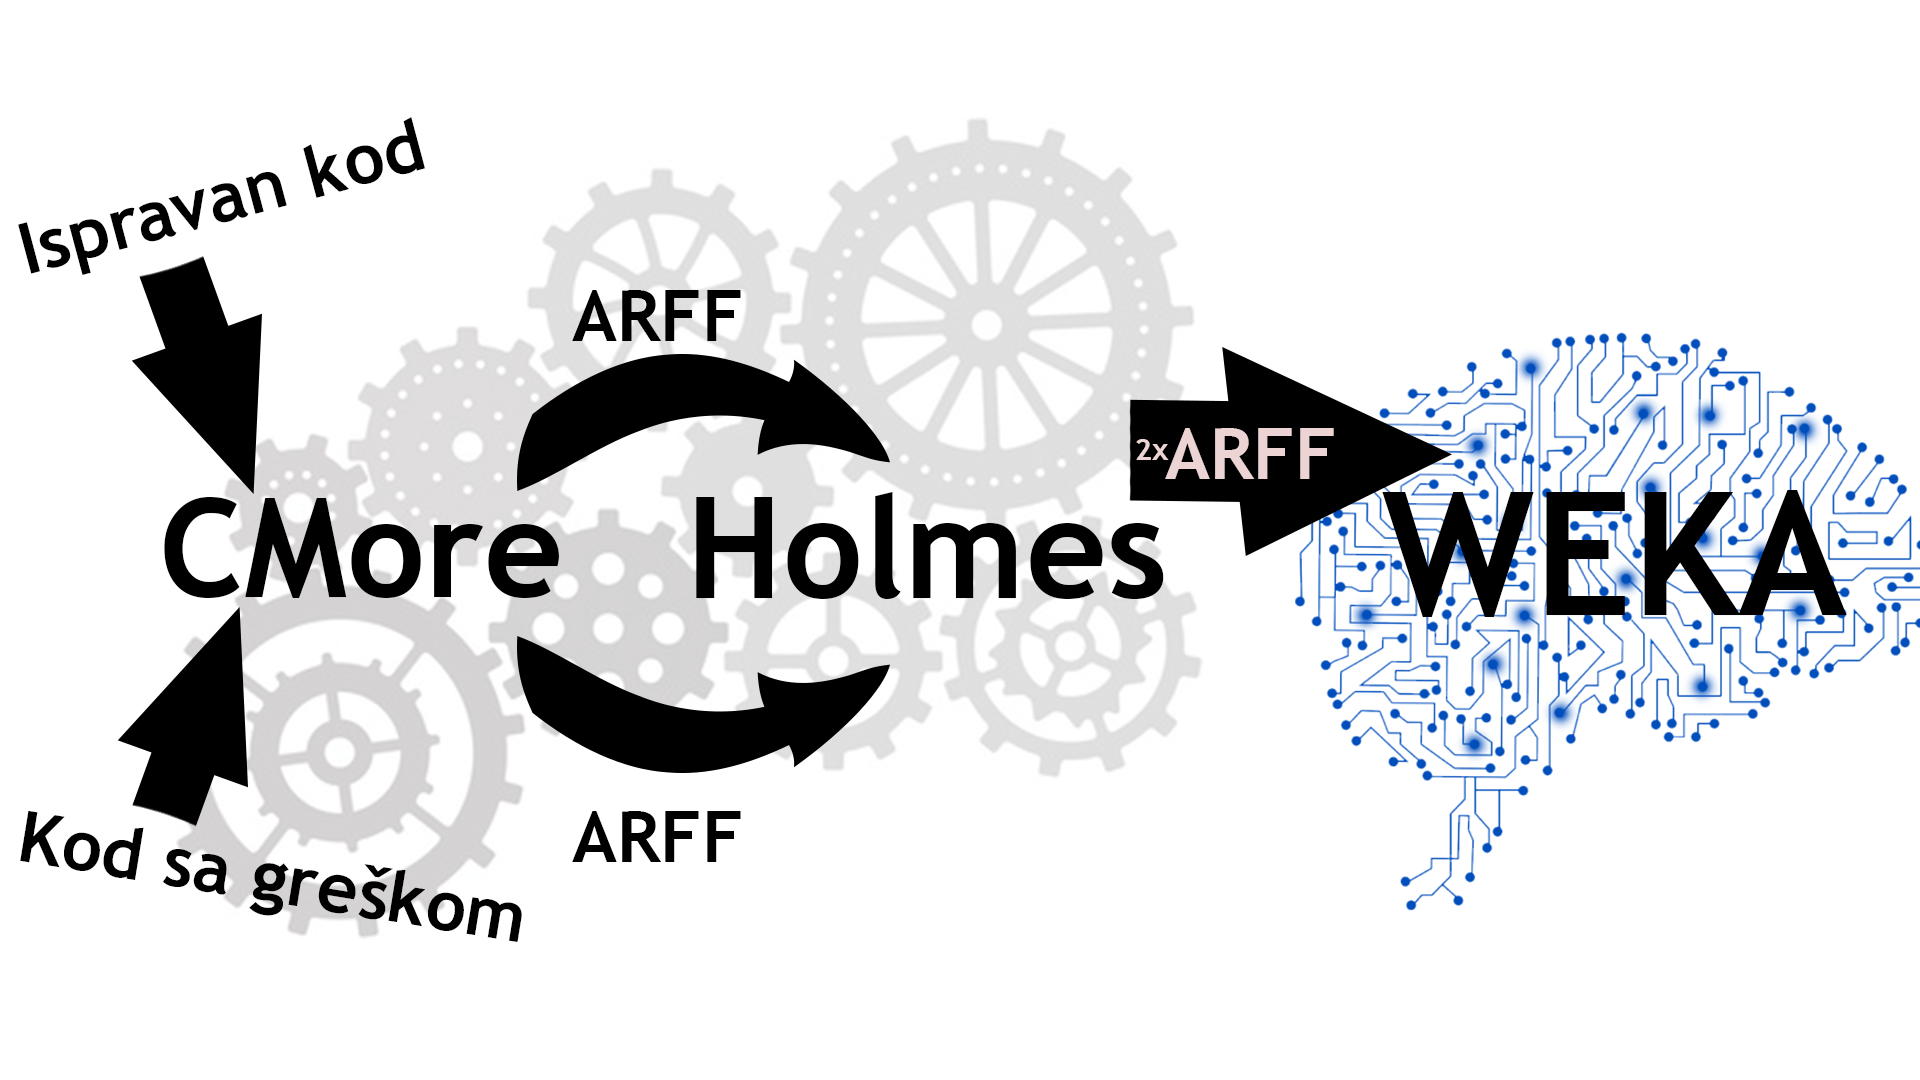
\includegraphics[width=\paperwidth, trim=0cm 0 0 -7cm]{weka.png}}
\begin{frame}
\end{frame}
}

\begin{frame}
\frametitle{Od izvornog koda do istreniranih modela}
\begin{itemize}


\item \textcolor{red}{WEKA} --- biblioteka mašinskog učenja
\item Jedna ARFF datoteka kao ulaz za više algoritama

\item Analiza pogodnosti daje rezultate poređenja 71 klasifikatora

\item Među najboljima su:
\begin{itemize}
	\item Neuronska mreža MultiLayerPerceptron
	\item Najbliži susedi Ibk
	\item Stabla ADABoost(BFTree)
\end{itemize}
\end{itemize}
\end{frame}

\subsection{Onlajn testiranje korišćenjem učenja uslovljavanjem}
\label{subsec:online-rl}
\begin{frame}
\frametitle{Onlajn testiranje}

\begin{itemize}
	\item Veliki, nedeterministički sistemi?
	\item Kombinovanje generisanje testova i njihovo izvršavanje
	\item Pokriva najrelevantnija ponašanja
	\item Testiranja bazirana na modelu (eng. \textcolor{red}{model-based testing})
	\begin{itemize}
		\item Implementacija pod testom \newline (eng. \textcolor{red}{implementation under test --- IUT})
		\item Model	
	\end{itemize}
\end{itemize}

\end{frame}

\begin{frame}
\frametitle{Onlajn testiranje}

\begin{itemize}
	\item Akcije testera --- kontrolisane akcije
	\item Akcije IUT --- posmatrane akcije


\item Pravila ažuriranja:
\begin{itemize}
	\item $[[p]] \subseteq Stanja \times Vrednost^n \times Stanja$
	\item $[[p]] \subseteq Stanja \times Vrednost^n \rightarrow Stanja$
\end{itemize}

\item Čuvano pravilo ažuriranja je par ($\varphi$,p) 
\end{itemize}
\end{frame}


\begin{frame}
\frametitle{Onlajn testiranje}

Izbor naredne akcije:
\begin {itemize}
	\item Ukoliko nema mogućih akcija: \newline \textbf{prekini trenutni test}
	\item Ukoliko nema mogućeg izbora za kontrolisanu akciju: \newline \textbf{vrati posmatranu}
	\item Ukoliko nema mogućeg izbora za posmatranu akciju: \newline \textbf{vrati kontrolisanu}
	\item Inače: \newline \textbf{izaberi između kontrolisane i posmatrane akcije}
\end {itemize}

\end{frame}

\begin{frame}
\frametitle{Onlajn testiranje}

\begin{itemize}
\item Politika izbora:
\begin{itemize}
	\item Najjeftinija
	\item Nasumična
	\item Najmanje frekventna
\end{itemize}
\item \textbf{Učenje uslovljavanjem, anti-ant algoritam}
\item Akcije $(a_i)_{i < k}$, Cene $(c_i)_{i < k}$
\item Verovatnoća za izbor akcije $a_i$ je $c_i^{-1} / \sum_{j=0}^{k} c_j^{-1}$
\end{itemize}
\end{frame}

\section[]{Zaključak}
\label{sec:zakljucak}
\begin{frame}
\frametitle{Zaključak}
\begin{itemize}
\item Značaj verifikacije softvera
\item Izuzetno dobri rezultati tehnika mašinskog učenja
\item Prirodno je razmišljati o primeni mašinskog učenja na verifikaciju softvera
\item Primene i u statičkoj i u dinamičkoj verifikaciji
\item Odabrane primene:
	\begin{itemize}
		\item Formalna verifikacija
		\item Učenje statičkog analizatora iz podataka
		\item Od izvornog koda do istreniranih modela
		\item Onlajn testiranje korišćenjem učenja uslovljavanjem
	\end{itemize}
\end{itemize}
\end{frame}

\section[]{Literatura}
\begin{frame}
\frametitle{Literatura}
\begin{itemize}
\item Lutz Hamel, On the use of machine learning in formal software verification, University of Rhode Island, 2003.
\item Christopher M. Bishop, Pattern Recognition and Machine Learning (Information Science and Statistics), Springer-Verlag New York, Inc, Secaucus, NJ, 2006.
\item Hannes Tribus, Static Code Features for a Machine Learning based Inspection, School of Engineering, Blekinge Institute of Technology, Sweden, 5 2010.
\item Margus Veanes, Pritam Roy and Colin Campbell, Online testing with reinforcement learning, In Formal Approaches to Software Testing and Runtime Verification, FATES/RV 2006, volume 4262, Springer Verlag, January 2006.
\end{itemize}
\end{frame}

\begin{frame}[plain]
\centering\Huge{Hvala na pažnji!}
\end{frame}

\end{document}